\Chapter{Tervezés}

A szimulációs környezet megfelelő működéséhez el kell tárolnunk az ágensek és a mapot összeállító blockok adatait.
Ennek a megvalósításához szükséges leírni mely adatokat kell eltárolnunk és adatmodelleket készítése is elegedhetetlen az átláthatóságért.

\section{Adatmodellek}

\begin{figure}[!ht]
	\centering
	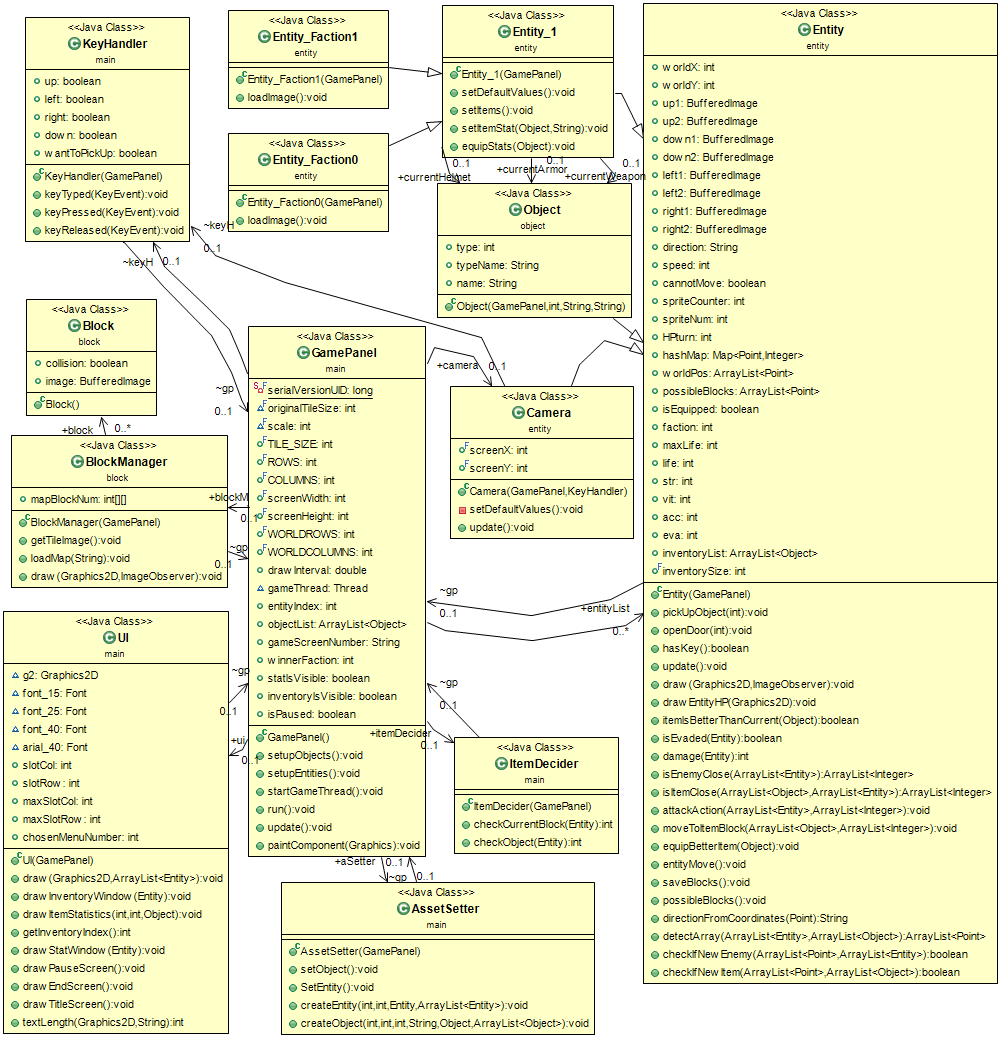
\includegraphics[scale=0.45]{images/UML.png}
	\caption{UML}
	\label{fig:UML}
\end{figure}